Generating vectors are used by the lattice generators to compute point sets. Previous works \cite{Kor59,Slo02,KuoJoe02b,NuyCoo06a} commonly applied greedy component-by-component (CBC) algorithms to construct generating vectors. However, this process is dependent on weight vectors and the decay of Fourier coefficients. To this end, Takashi Goda and Pierre L'Ecuyer suggested in their work \cite{doi:10.1137/22M1473625} that generating vectors do not require a predetermined weight vector and a  measure of the decay of Fourier coefficients to reach a high precision; instead, random generators can also achieve desirable results. Recently, we implemented random generating vectors into QMCPy, and the results were quite promising. This blog will explore the usage of random generating vectors in QMCPy through code examples. Before that, however, we shall  consider some mathematics behind generating vectors. 

\subsection*{Mathematics of generating vectors}

Given $N>2$ and generating vector $z \in \{1,\dots,N-1\}^d$, define $P_N := P_{N,z}$ where 
\begin{equation*}
    x_n = \left\{\frac{nz}{N}\right\}, n = 0,1,\dots,N-1,
\end{equation*}
where $\{s\} = s-\lfloor s \rfloor$ denotes the fractional part of each component. The significance of the generating vector is that it determines the point set $P_N = \{\boldsymbol{x_0},\boldsymbol{x_1},\dots,\boldsymbol{x_{N-1}}\} \subset [0,1)^d$ for given $N$.  

The following are plots of lattices generated by QMCPy when $N$ is a power of 2:
\begin{figure}[H]
    \centering
    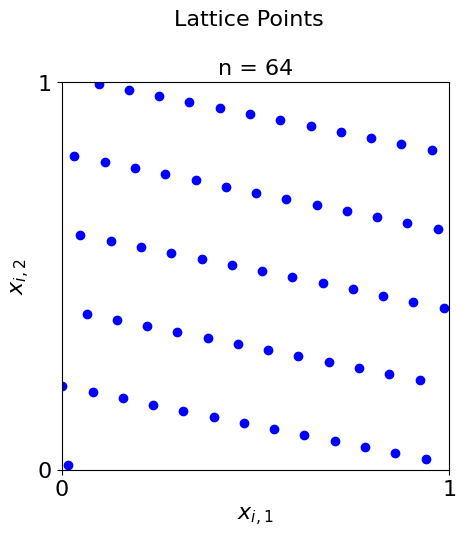
\includegraphics[width=0.18\linewidth]{TotallyRandomLattice/Figures/1.png}
    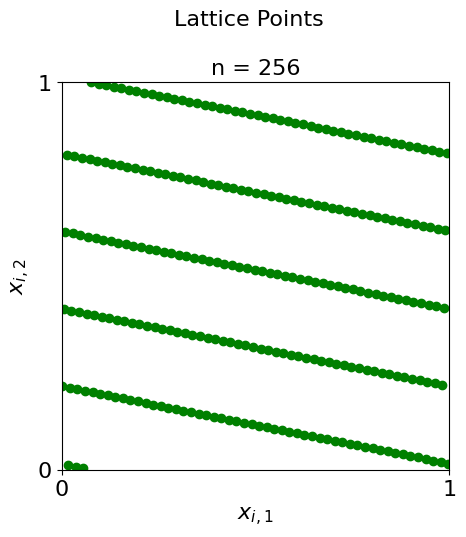
\includegraphics[width=0.18\linewidth]{TotallyRandomLattice/Figures/2.png}
    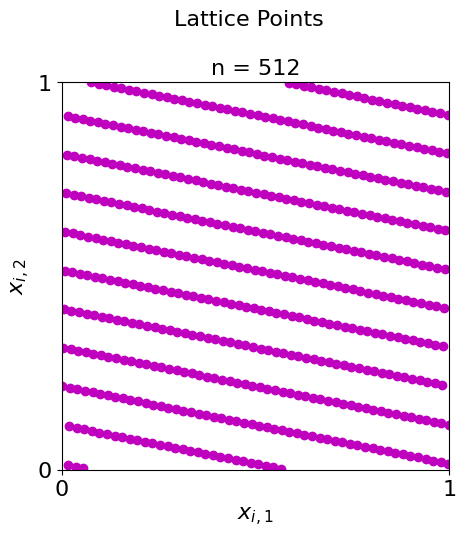
\includegraphics[width=0.18\linewidth]{TotallyRandomLattice/Figures/3.png}
    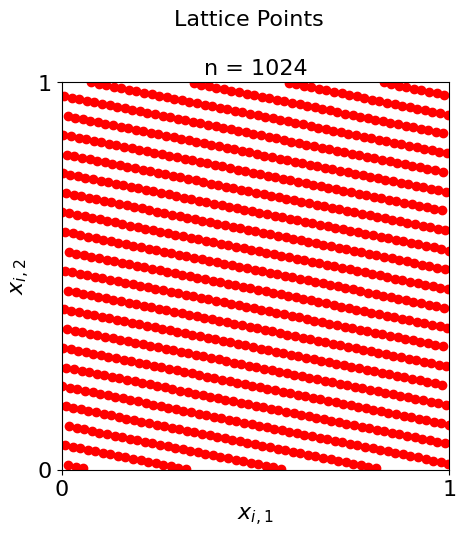
\includegraphics[width=0.18\linewidth]{TotallyRandomLattice/Figures/4.png}
    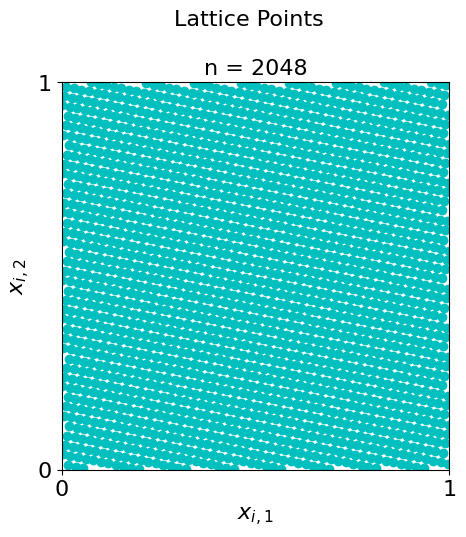
\includegraphics[width=0.18\linewidth]{TotallyRandomLattice/Figures/5.png}
    \caption{lattices generated using $generating\_vector = 16$ and $seed = 136$. These plots can be conditionally reproduced using \code{lattice\_random\_generator.ipynb}}
    \label{fig:lat_pts}
\end{figure}

While samples in \cite{doi:10.1137/22M1473625} were produced by a prime sample size, QMCPy utilizes sample sizes that are powers of 2 due to its expectation of extensible generating vectors. 
The usage of the generating vector comes from the Quasi-Monte Carlo integration using a point set $P_N$:
\begin{equation*}
    I(f) := \int_{[0,1)^{d}} f(x)dx \approx I(f;P_N) = \frac{1}{N}\sum_{n=0}^{N-1} f(x_n)
\end{equation*}

In their work, Goda and L'Ecuyer approximated $I(f)$ by the median rules: $\textrm{median}(I(f;P_{N,\ z_1}),\dots,I(f;P_{N,z_r}))$ \cite{doi:10.1137/22M1473625}, while while QMCPy utilizes mean rules: $\textrm{mean}(I(f;P_{N,z_1}),\dots,I(f;P_{N,z_N}))$. We performed numerical experiments in the final section to have a glimpse on the efficiency of both rules. 

\subsection*{Code examples}
In this section, we will explore the basic features of the \verb|Lattice| Class and the \verb|gen_samples| method. For further documentation, please resort to \href{https://qmcpy.readthedocs.io/en/latest/algorithms.html#module-qmcpy.discrete_distribution.lattice.lattice}{QMCPy Lattice Documentation}.

The generating vector is the core of the \verb|Lattice| object. Currently, QMCPy enables the following types of cubature schemes:

\begin{enumerate}
    \item A hard-coded n-dimensional array. 
    \item A file that contains a hard-coded generating vector
    \item A totally random generator produced by integer input
\end{enumerate}

We will focus on the recently-developed third type of generating vectors because it is a direct application of the mathematics discussed above. 

\subsubsection*{Lattice declaration and the gen\_samples function}

A \verb|Lattice| object in QMCPy requires the dimension and the generating vector of choice. Other arguments such as randomize or seed are optional. 

The following code is a short example used to illustrate the declaration of a \verb|Lattice| object and the \verb|gen_samples| function.

\lstinputlisting[style=Python]{TotallyRandomLattice/code/lattice_initialization.py}

The output is listed below:

\lstinputlisting[frame = tlrb]{TotallyRandomLattice/code/latticeinitout.out}

\pagebreak

\subsubsection*{Integration}

To integrate in QMCPy, one needs to declare the dimension, the tolerance, a low discrepancy sequence, and the true measure used to transform the object function to the $d$ dimensional unit cube. In the following example, the Gaussian measure is applied using a lattice as the low discrepancy sequence. The Keister function \cite{Kei96}, is used as an example. 



\lstinputlisting[style=Python]{TotallyRandomLattice/code/integration.py}



\noindent\begin{minipage}{.45\textwidth}
\lstinputlisting[caption = random generator,frame = tlrb]{TotallyRandomLattice/code/integraloutrandom.txt}
\end{minipage}\hfill
\begin{minipage}{.45\textwidth}
\lstinputlisting[caption = default generator,frame = tlrb]{TotallyRandomLattice/code/integraloutdefault.txt}
\end{minipage}

One can see that the default generator performs slightly better than the random generator as the time to integrate is about $0.16$ seconds lower. 

\pagebreak



\subsection*{Comparison between lattice generators}
To have a further glimpse into the performance of lattice generators, we compared the error of three types random generators with respect to the sample size. The blue line depicts a random generator that applies the median rule $\mathrm{median}(I(f;P_{N,z_1}),\dots,I(f;P_{N,z_r}))$; the orange depicts a generator that applies the mean rule $\mathrm{mean}(I(f;P_{N,z_1}),\dots,I(f;P_{N,z_r}))$; the green is a randomly shifted hard-coded generator. 


 \begin{figure}[H]
    \centering
    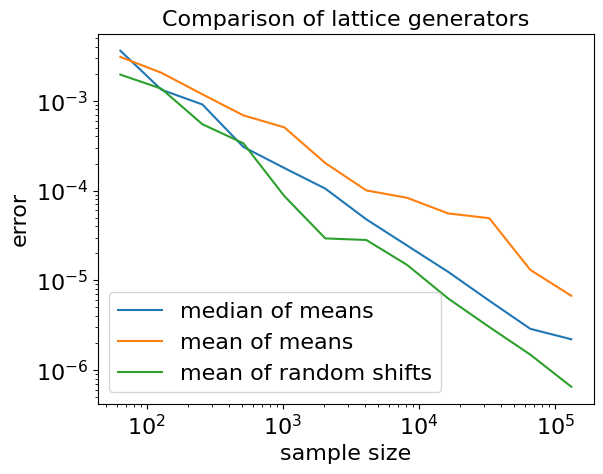
\includegraphics{TotallyRandomLattice/Figures/meanvsmedian.png}
    \caption{A comparison between lattice generators. This plot can be conditionally reproduced using \code{lattice\_random\_generator.ipynb}}
\end{figure}

Here, we used sample sizes $N$ ranging from $2^6$ to $2^{18}$ and $r = 11$. We compared the results of integrating the 2-dimensional Keister integral over each sample size using each type of lattice generator. To reduce sampling variance, we repeated the trails $25$ times and computed the averaged result. 

As shown in the plot, mean of random shifts (green) outperforms the random generator using median rules (blue), which in turn outperforms the random generator using mean rules (orange). These results support findings in \cite{doi:10.1137/22M1473625}. More numerical experiments under difference circumstances should be conducted before making a conclusion, but current works suggest that random lattice generators have a lot of potential 



